%%%%%%%%%%%%%%%%%%%%%%% file template.tex %%%%%%%%%%%%%%%%%%%%%%%%%
%
% This is a general template file for the LaTeX package SVJour3
% for Springer journals.          Springer Heidelberg 2010/09/16
%
% Copy it to a new file with a new name and use it as the basis
% for your article. Delete % signs as needed.
%
% This template includes a few options for different layouts and
% content for various journals. Please consult a previous issue of
% your journal as needed.
%
%%%%%%%%%%%%%%%%%%%%%%%%%%%%%%%%%%%%%%%%%%%%%%%%%%%%%%%%%%%%%%%%%%%
%
% First comes an example EPS file -- just ignore it and
% proceed on the \documentclass line
% your LaTeX will extract the file if required
\begin{filecontents*}{example.eps}
%!PS-Adobe-3.0 EPSF-3.0
%%BoundingBox: 19 19 221 221
%%CreationDate: Mon Sep 29 1997
%%Creator: programmed by hand (JK)
%%EndComments
gsave
newpath
  20 20 moveto
  20 220 lineto
  220 220 lineto
  220 20 lineto
closepath
2 setlinewidth
gsave
  .4 setgray fill
grestore
stroke
grestore
\end{filecontents*}
%
\RequirePackage{fix-cm}
%
%\documentclass{svjour3}                     % onecolumn (standard format)
%\documentclass[smallcondensed]{svjour3}     % onecolumn (ditto)
\documentclass[smallextended]{svjour3}       % onecolumn (second format)
%\documentclass[twocolumn]{svjour3}          % twocolumn
%
\smartqed  % flush right qed marks, e.g. at end of proof
%
\usepackage{graphicx}

%
% \usepackage{mathptmx}      % use Times fonts if available on your TeX system
%
% insert here the call for the packages your document requires
%\usepackage{latexsym}

\usepackage{natbib} % delete before submission
\bibliographystyle{plain} % delete before submission
\usepackage{amsmath, amssymb}
\usepackage{algorithm}
\usepackage{algorithmic}
%\usepackage[noend]{algpseudocode}

%\usepackage{hyperref}

\newcommand{\x}{\item}
\DeclareMathOperator{\E}{\mathbb{E}}

% please place your own definitions here and don't use \def but
% \newcommand{}{}
%
% Insert the name of "your journal" with
% \journalname{myjournal}
%
\begin{document}
\title{Reviewing and improving Natural Actor Critic methods
%\thanks{Grants or other notes
%about the article that should go on the front page should be
%placed here. General acknowledgments should be placed at the end of the article.}
}
% \subtitle{Do you have a subtitle?\\ If so, write it here}

%\titlerunning{Short form of title}        % if too long for running head

\author{Maximilian A. Gehrke\and\\Yannik P. Frisch\and Tabea A. Wilke
}

%\authorrunning{Short form of author list} % if too long for running head

\institute{Maximilian A. Gehrke \at
              TU Darmstadt, Germany\\
              \email{maximilian\_alexander.gehrke@stud.tu-darmstadt.de}           %  \\
%             \emph{Present address:} of F. Author  %  if needed
           \and
           Yannik P. Frisch \at
           TU Darmstadt, Germany\\
           \email{yannik\_phil.frisch@stud.tu-darmstadt.de}
           \and
           Tabea A. Wilke \at
           TU Darmstadt, Germany\\
           \email{tabeaalina.wilke@stud.tu-darmstadt.de}
}
\date{Received: date / Accepted: date}
% The correct dates will be entered by the editor
\maketitle

 % ------------------------------ TASKS -------------------------------------- %
 
% (1) Formality & Language: The report uses the LaTex template and does not exceed 8 pages + 2 pages references. The report is understandable and does not contain any typos, slang or any other errors [10 points]
% (2) Structure & Figures: The report is well structured and has a coherent story that integrates the individual papers known from literature into a bigger picture. Figures and diagrams are well described, labeled, and informative. [10 points]
% (3) Overview: The report provides an extensive overview about the existing literature and provides a summary of the algorithm/platform, variations thereof and its applications [15 points]
% (4) Discussion & Contribution: Besides summarizing, the report compares the existing literature and highlights the differences between approaches. Thereby, introducing a new perspective / overview, which is not present in current literature.

 % ------------------------------- Abstract ---------------------------------- %
\newpage
\begin{abstract}
In this paper we describe the natural actor critic approach and provide an extensive overview about the current research. This includes a basic description of the natural gradient, actor critic approaches and comparisons between existing extensions. Additionally, we improve the episodic Natural Actor Critic algorithm by applying it with two neural networks instead of basis functions.


% FÜR PROJECT: Our implementation is very basic that can be extended arbitrarily granular. The emphasis of this paper is a detailed description of the implementation process and how it can be used. Results are reported for several of the standard reinforcement learning problems, using the publicly available gym library.

\keywords{Natural Gradient \and Neural Networks \and Advantage Function}
% \PACS{PACS code1 \and PACS code2 \and more}
% \subclass{MSC code1 \and MSC code2 \and more}
\end{abstract}


% ---------------------- Introduction --------------------------------- %
\newpage
\section{Introduction}
\label{intro}

In reinforcement learning, more wider, in machine learning, policy gradient methods have dominated the field in the last years. Python machine learning libraries like keras, tensorflow or PyTorch are used for implementing neural networks, which are trained using the policy gradients of the weights. These methods aim to maximize an objective function $J(\Theta)$ by repeatedly calculating the gradient of the policy w.r.t. the parameters and updating the parameters in that direction.

\begin{equation}
\label{equ:polupdate}
\Delta_{\Theta} = \alpha \nabla_{\Theta} J(\Theta)
\end{equation}

\noindent Simple calculus tells us that the gradient is the steepest direction so eventually this method will converge to a local maximum. So how do we get the gradient of the objective function $J(\Theta)$ w.r.t. the parameters $\Theta$? Applying some transformations and the likelihood-ratio trick, we obtain the policy gradient theorem, which gives us the gradient of the objective function:

\begin{equation}
	\label{equ:policygradienttheorem}
	\nabla_{\Theta}J(\Theta)=\E_{\pi_{\theta}}[\nabla_{\theta}\log\pi_{\theta}(a|s) Q^{\pi_{\theta}}(s, a)]
\end{equation}

\noindent In the most basic policy gradient algorithm, REINFORCE, the action-value function $Q^{\pi_{\theta}}$ uses the return. 

\subsection{Applications}
NAC algorithms have been applied in various fields such as road traffic optimisation \cite{richter2007natural}, robotic control tasks \cite{kim2010impedance}, motor primitive learning \cite{peters2007applying} and ocomotion of a Two-Linked Robot Arm \cite{park2005rls}.


\subsection{Actor - Critic}

However, we can also take any other admissible estimator. Estimating the action-value function with a compatible function approximation $Q_w(s,a)$ \cite{sutton2000policy} is called a critic. This reduces variance because we do not have to roll out the complete episode to update our parameters. We can rather apply a TD like update after one or arbitrarily many steps.

Further, we can introduce a baseline. This does not change the expected value and further reduces our variance. Equation \ref{equ:policygradienttheorem} redefines to:

\begin{equation}
\label{equ:policybaseline}
\nabla_{\Theta}J(\Theta)=\E_{\pi_{\theta}}[\nabla_{\theta}\log\pi_{\theta}(a|s) Q_w(s, a) - B(s,a)]
\end{equation}

where $B(s, a)$ defines the baseline. A good baseline is in many cases the value function of the network. If we take the action-value function and reduce it by the value function, we are left with the advantage. In other words, we can immediately estimate the advantage function $A_w(s,a)$, which we will do throughout this paper. Equation \ref{equ:policybaseline} changes to:

\begin{equation}
	\nabla_{\Theta}J(\Theta)=\E_{\pi_{\theta}}[\nabla_{\theta}\log\pi_{\theta}(a|s) A_w(s, a)]
\end{equation}

\subsection{MDP}
- MDP\\
- Stochastic states/actions

\section{Natural Gradient}

The natural gradient was first introduced by Amari in 1998 \cite{amari1998natural}. The main difference between the natural gradient and the ordinary stochastic gradient method, is the direction it points to. Despite many expectations, the ordinary gradient does not always point to the steepest direction, especially not if the parameter space has a Riemann metric structure and is not Euclidean. For example, the parameter space of neural networks has been shown to exhibit a Riemannian character.

In comparison to vanilla gradient methods, the natural gradient finds the steepest direction for Riemannian parameter spaces. It utilizes the $n \times n$ matrix $G = (g_{ij})$, called the Riemannian metric tensor, which in general depend on $\theta$. The natural gradient is defined as

\begin{equation}
	\widetilde{\nabla}_{\theta} J(\theta) = G^{-1} \nabla_\theta J(\theta)
\end{equation}

where $\widetilde{\nabla}_{\theta}$ is the natural gradient w.r.t the parameters $\theta$.  Learning should be carried out with an update rule:

\begin{equation}
	\theta_{t+1} = \theta_{t+1} + \alpha \widetilde{\nabla}_{\theta} J(\theta)
\end{equation}

In the special case that the parameter space is Euclidean and the coordinate system is orthonormal, the conventional gradient equals the natural gradient:

\begin{equation}
	\widetilde{\nabla}_{\theta} J(\theta) = \nabla_{\theta}
\end{equation}

The natural gradient is the steepest ascent direction of our performance object with respect to any metric. Well, but how do we calculate the matrix $G$? The Hessian $H$ at $x_0$ (which exists since the first derivative vanishes) is the purely covariant form of the Riemann curvature tensor. To estimate the Hessian $H$, we can use the Fisher information metric 

\begin{equation}
	F_\theta=\E_{s\sim\rho^{\pi},a\sim\pi_{\theta}}\left[\nabla_{\theta}log\pi_{\theta}(a|s)^{T}\nabla_{\theta}log\pi_{\theta}(a|s)\right]
\end{equation}

\noindent For deterministic policies: 

\begin{equation}
	M_{\mu}(\theta)=E_{s\sim\rho^{\mu}}[\nabla_{\theta}\mu_{\theta}(s)\nabla_{\theta}\mu_{\theta}(s)^{T}w]
\end{equation}
\noindent$\rightarrow$ Limiting case of the Fisher information metric: policy variance reduced to zero


\noindent Combining DPG theorem with compatible function approximation gives 
\begin{equation}
\nabla_{\theta}J(\mu_{\theta}) = E_{s\sim\rho^{\mu}}[\nabla_{\theta} \mu_{\theta}(s) \nabla_{\theta} \mu_{\theta}(s)^{T}w]
\end{equation} 

\noindent so steepest ascent direction reduces to

\begin{equation}
M_{\mu}(\theta)^{-1}\nabla_{\theta}J_{\beta}(\mu_{\theta})=w
\end{equation} 


% ---------------------- Properties --------------------------------- %
\newpage
\section{Properties of the natural gradient}

\subsection{Online}
The natural gradient can be used online. This means that we can learn from incomplete sequences and reduce the variance. It is also possible to use an offline, episodic variant of the natural gradient which can be seen in section ??. With both variations at hand, one can make the decision regarding the structure of our problem. \cite{pascanu2013revisiting, peters2008natural}

\subsection{1st order method}
The natural gradient is a first order method, but implements many second order advantages \cite{pascanu2013revisiting}. This is especially relevant for problems,  where the access to the cost function is only indirect possible. For example Deep Boltzmann Machines exhibit this characteristics and recent studies showed possible solutions with NG \cite{desjardins2013metric} whereas second order  methods are hard to apply.

\subsection{Parametrization invariant}
The natural gradient is invariant regarding parametrization. This comes from the KL-divergence constraint we apply, which measures the changes of our probability density estimation regardless how it was parametrized \cite{pascanu2013revisiting}. This is comparable to signal noise whitening \cite{sohl2012natural}.

\subsection{Faster convergence}
In many cases natural gradient algorithms converge faster than vanilla gradient algorithms. \cite{sohl2012natural, ??, ??}. This is due to the fact, that a metric is used which removes the dependencies and differences in scaling between the parameters. This means, that the parameters are perpendicular to each other and the parameter space can be explored more efficiently \cite{sohl2012natural}.

% ---------------------- Extensions --------------------------------- %
\newpage
\section{Extensions}

\subsection{Episodic NAC}

\subsection{Fitted NAC}

Fittet natural actor critic (FNAC) is a fitted version of the natural actor critic algorithm described in section \ref{?} \cite{melo2008fitted}.  It allows the utilization of general function approximations and efficient data reuse. This combination is especially appealing, because it combines the faster convergence properties of natural gradient algorithms with the efficient data use of regression algorithms.

\subsection{Importance Sampling}

Melo et. al additionally implemented importance sampling, which increased the efficient use of data even further \cite{melo2008fitted}.

\subsection{Incremental NAC}

\subsection{Implicit incremental NAC}

\subsection{Regularization on NAC}
	Even if we find the inverse of $G$, it can be ill defined. An example for this are extremely small eigenvalues which appear due to noise in our data. These eigenvalues will become extremely large if we take the inverse of $G$ and thus the parameters belonging to the eigenvalues will get a lot of credibility which they should not have and which will falsify our inverse.
	
	That is why there have been some approaches to introduce a regularization term \cite{sohl2012natural}. Regularizing the matrix inverse can for example be done by a technique called stochastic robust approximation \cite{boyd2004convex}, where $G^{-1}$ is replaced by 
	
	\begin{equation}
		G^{-1}_{\text{reg}} = \left( G^T G + \epsilon I \right)^{-1} G^T
	\end{equation}
	
	\noindent where $\epsilon$ denotes for a small constant (e.g 0.01).
	
	Another idea is the application of ridge regression \cite{hoerl1970ridge}, which has a build in regularizer. We can calculate $\widetilde{\nabla}_{\theta} J(\theta)$ by solving the linear equation
	
	\begin{equation}
		G(\theta) \widetilde{\nabla}_{\theta} J(\theta) = \nabla_{\theta} J(\theta)
	\end{equation}
	
	\noindent in the direction of $\widetilde{\nabla}_{\theta} J(\theta)$.
	
	Witsch et al. use an approach similar to least squares regularization \cite{witsch2011enhancing}. 
	
	\begin{equation}
		\widetilde{\nabla}_{\theta} J(\theta) = \left( F + \lambda I \right)^{-1} \nabla_\theta J(\theta)
	\end{equation}
	
	\noindent If $\lambda$ is huge, the Fisher matrix only has a small influence on the change in direction. Therefore, we want to scale $\lambda$ regarding $F$:
	
	\begin{equation}
		\lambda = \dfrac{\alpha}{\text{det}(F) + 1}
	\end{equation}

	\noindent with $\alpha$ a small constant, e.g. $0.01$.
	
	
	\subsection{POMDPs}
	There have been some approaches to apply the NAC to POMDPS. A promising approach is the Natural Actor and Belief Critic \cite{jurvcivcek2011natural}, which learns parameters in statistical dialogue systems. These can be modeled as POMDPs.
	
	\subsection{Least Squares}
	
	Recursive least squares: \cite{park2005rls}

% ---------------------- Improvements --------------------------------- %
\newpage
\section{Improvements}

% ---------------------- Discussion --------------------------------- %
\newpage
\section{Discussion}

Some sources claim that the eNAC and the NAC-LSTD algorithms use a biased estimate of the natural gradient \cite{thomas2014bias}.


% -------------------- Paper ----------------------- %
\newpage
\section{Paper}
Natural Actor Critic:
\begin{itemize}
	\item Main Version \cite{peters2005natural}.
	\item 2nd Version: Natural Actor-Critic in Neurocomputing \cite{peters2008natural}.
	\item 3rd version: RL of motor skills with policy gradients in NN \cite{peters2008reinforcement}.
\end{itemize}

\noindent Must read paper to understand basics by Jan:
\begin{itemize}
	\item Policy Evaluation with TD \cite{dann2014policy}.
\end{itemize}

\noindent Recommended by Jan:
\begin{itemize}
	\item Incremental NAC algorithms \cite{bhatnagar2008incremental}.
	\item Jan said that a paper form C. Dann is very important. Did he mean Policy Evaluation with TD by Dann or did he mean a second paper?
\end{itemize}

\noindent Research:
\begin{itemize}
	\item Comparison of four natural gradient algorithms (co-author Sutton) \cite{bhatnagar2009natural}.
\end{itemize}

% -------------------- Mettings & Notes ----------------------- %
\section{Meetings \& Notes}

Meetings:
\begin{itemize}
	\item 12.12.18: Notes from Jan can be found in ``.\textbackslash Notes Jan 12.12.18''
\end{itemize}

% ---------------------- eNAC --------------------------------- %

\section{Ideas}
\subsection{Fitted NAC}

\begin{align}
	\pi(a|s) = p(a|s, \Theta) = \mathcal{N}(a|\mu = NN_{\Theta}(s), \sigma) \\
	f(s,a) = \log p(a|s, \Theta)^T w \\
	f_V(s) = NN_V(s) \\
	\text{''fitted''}\\
	\min_{V_t, W_t} (r(s,a) + \gamma f_{V_{t+1}}(s') - f_{V_t}(s) + f_{W_t}(s,a))^2
\end{align}



\subsection{Ideas of TRPO}


\subsection{Other Extentions}

\begin{itemize}
	\x stochastic
	\x minibatches
	\x importance sampling:
\end{itemize}

\begin{align}
	V_{\Theta} J = \sum \mu(s) \pi'(a|s) \nabla \log \pi'(a|s) Q^{\pi'}(a|s) \\
	\approx \dfrac{1}{N} \sum \nabla \log \pi'(a|s) Q(s,a) = g(\Theta)
\end{align}





\section{Episodic NAC}
Important to understand beforehand: In episodic NAC, our system of equations has one equation per trajectory and not one equation per action as in the normal NAC algorithm.
\\\\
First we start by adding together the advantage function across an episode $e$ where we made $N$ steps.

\begin{align}
	A(s,a) &= r(s,a) + \gamma V(s') - V(s) \\
	\gamma A(s',a') &= \gamma r(s', a') + \gamma^2V(s'') - \gamma V(s') \\
	A(s, a) + \gamma A(s', a') &= r(s,a) + \gamma r(s',a') + \gamma^2 V(s'') - V(s) \\
	\sum_{i = 0}^{N}\gamma^i A(s_i, a_i) &= \sum_{i = 0}^{N}\gamma^i r(s_i, a_i) + \gamma^N V(S_{N+1}) - V(S_0)
\end{align}

\noindent If we assume $\gamma \neq 1$, we can remove the term $\gamma^N V(S_{N+1})$, because in the limit the term becomes zero ($\gamma^N \rightarrow 0$). Additionally, if we assume that we always start in the same start $S_0$, we can write $V(S_0)$ as our cost function $J$ because it will exactly sum up the expected Reward/cost of our problem.

\begin{equation}
	\Rightarrow \sum_{i = 0}^{N}\gamma^i A(s_i, a_i) = \sum_{i = 0}^{N}\gamma^i r(s_i, a_i) - J
\end{equation}

\noindent Now we can plug in the parametrisized gradient descent for the advantage function. That this works and is indeed the same has been proven by \underline{reference}. Additionally we bring the cost $J$ to the other side of the equation.

\begin{equation}
	\label{equ:someequ}
	\Rightarrow \sum_{i = 0}^{N} \gamma^i \nabla_{\Theta} \left[\log \pi(a_i | s_i)^T\right] \cdot w + 1 \cdot J = \sum_{i = 0}^{N}\gamma^i r(s_i, a_i)
\end{equation}

\noindent Let's do some rewriting. We define the following two terms:
\begin{align}
	\Phi_e = \left[  \sum_{i = 0}^{N} \gamma^i \nabla_{\Theta} \left[\log \pi(a_i | s_i)^T\right] , 1 \right]\\
	R_e = \sum_{i = 0}^{N}\gamma^i r(s_i, a_i)
\end{align}

\noindent This let's us rewrite equation \ref{equ:someequ} as:

\begin{equation}
	\Phi_e \cdot \begin{bmatrix} w\\J \end{bmatrix}  = R_e
\end{equation}

\noindent An easy way to solve this system of equations is by taking the pseudo inverse of $\Phi_e$.

\begin{equation}
	\begin{bmatrix} w\\J \end{bmatrix} = (\Phi_e^T \Phi_e)^{-1} \Phi_e^T R_e
\end{equation}

\begin{algorithm}
	\caption{Episodic Natural Actor-Critic Algorithm (eNAC)}\label{euclid}
	\begin{algorithmic}
		\REQUIRE $n \geq 0 \vee x \neq 0$
		\ENSURE $y = x^n$
		\FOR{$u = 1,2,3,\dots$}
			\FOR{$e = 1,2,3,\dots$}
				\STATE \textbf{Execute Rollout:} Draw initial state $s_0 \sim p(s_0)$
				\FOR{$t =1,2,3,\dots,N$}
					\STATE Draw action $u_t\sim\pi(a_t|s_t)$, observe next state $s_{t+1} \sim p(s_{t+1}|s_t, a_t)$, and reward $r_t = r(s_t, a_t)$.
				\ENDFOR
			\ENDFOR
		\ENDFOR
	\end{algorithmic}
\end{algorithm}



% ---------------------- How to use this template  --------------------------------- %

%\section{Section title}
%\label{sec:1}
%Text with citations \cite{RefB} and \cite{RefJ}.
%\subsection{Subsection title}
%\label{sec:2}
%as required. Don't forget to give each section
%and subsection a unique label (see Sect.~\ref{sec:1}).
%\paragraph{Paragraph headings} Use paragraph headings as needed.
%\begin{equation}
%a^2+b^2=c^2
%\end{equation}
%
%% For one-column wide figures use
%\begin{figure}
%% Use the relevant command to insert your figure file.
%% For example, with the graphicx package use
%  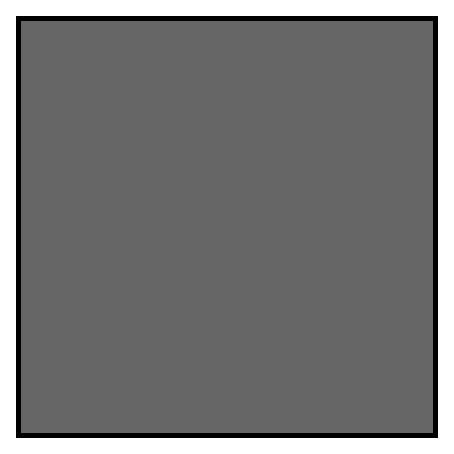
\includegraphics{example.eps}
%% figure caption is below the figure
%\caption{Please write your figure caption here}
%\label{fig:1}       % Give a unique label
%\end{figure}
%%
%% For two-column wide figures use
%\begin{figure*}
%% Use the relevant command to insert your figure file.
%% For example, with the graphicx package use
%  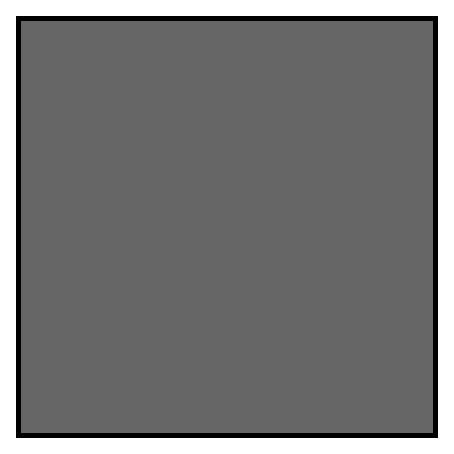
\includegraphics[width=0.75\textwidth]{example.eps}
%% figure caption is below the figure
%\caption{Please write your figure caption here}
%\label{fig:2}       % Give a unique label
%\end{figure*}
%%
%% For tables use
%\begin{table}
%% table caption is above the table
%\caption{Please write your table caption here}
%\label{tab:1}       % Give a unique label
%% For LaTeX tables use
%\begin{tabular}{lll}
%\hline\noalign{\smallskip}
%first & second & third  \\
%\noalign{\smallskip}\hline\noalign{\smallskip}
%number & number & number \\
%number & number & number \\
%\noalign{\smallskip}\hline
%\end{tabular}
%\end{table}

% -------------------- Acknowledgements ----------------------- %
%\begin{acknowledgements}
%If you'd like to thank anyone, place your comments here
%and remove the percent signs.
%\end{acknowledgements}



% -------------------- References ----------------------- %
% TODO: alle unten angegbenen Stile machen ganz komische Sachen
% Wer weiß, wie wir das fixen, bitte machen und oben \usepackage{natbib}
% und \bibliographystyle{plain} raus nehmen
% BibTeX users please use one of
%\bibliographystyle{spbasic}      % basic style, author-year citations
%\bibliographystyle{spmpsci}      % mathematics and physical sciences
%\bibliographystyle{spphys}       % APS-like style for physics
\bibliography{NAC-bibliography.bib}   % name your BibTeX data base

\end{document}

